\documentclass{beamer}

%\usepackage[UTF8,noindent]{ctex}
\usepackage{amsmath,amsxtra}
\usepackage{color}
\usepackage[version=3]{mhchem}
\usepackage{fixltx2e}
\usepackage{bbold}
\usepackage{mathrsfs}
%\usepackage{minted}
\usepackage{cleveref}
%\usepackage{mathtools}     
\usefonttheme{serif}
\usetheme{Warsaw}
\usecolortheme{orchid}
\usepackage{capt-of}
\usepackage{lmodern} % remove the warning for use of the \textit
\makeatletter
\renewcommand\normalsize{%
   \@setfontsize\normalsize\@xpt\@xiipt
   \abovedisplayskip 1\p@ \@plus2\p@ \@minus5\p@
   \abovedisplayshortskip \z@ \@plus3\p@
   \belowdisplayshortskip 6\p@ \@plus3\p@ \@minus3\p@
   \belowdisplayskip \abovedisplayskip
   \let\@listi\@listI}
\makeatother
\setbeamerfont{caption}{size=\tiny}
% \setbeamertemplate{caption}[numbered] %number the caption and change the font
% size

\newtheorem{thm}{Theorem}
\setlength\abovecaptionskip{0pt}
\usepackage{graphicx}
\graphicspath{{./figures/}}

\title{Accelerating Spark Shuffle with RDMA}
\author{
  Liu Bing\inst{1} \and Liu Fang\inst{2} \and Xiao Nong\inst{1} \and Chen Zhiguang\inst{1}
}
\institute{
  \inst{1}National University of Defense Technology \\
  \inst{2}Sun Yat-Sen University
}
\date{October 12, 2018}

\begin{document}

\begin{frame}[plain]
  \maketitle
\end{frame}

\AtBeginSection
{
	\begin{frame}
	\tableofcontents[
	currentsection,
	]
	\end{frame}
}

\section{Motivation}

\begin{frame}
  \frametitle{Shuffle Operations in Apache Spark}
  \begin{tabular}{ccc}
    $\overrightarrow{\mathbf{x}} = x_1, x_2, x_3, x_4$ &  & $\mathbf{A^{T}}\overrightarrow{\mathbf{y}} = \overrightarrow{\mathbf{0}}$ \\
    potential at nodes & & Kirchhoff\rq{s} Current Law \\
    \\
    $\overrightarrow{\mathbf{e}} = \mathbf{A^{T}}\overrightarrow{\mathbf{y}}~\downarrow$ & & $\uparrow~\mathbf{A^{T}}\overrightarrow{\mathbf{y}}$ \\
    \\
    $x_2 - x_1$, etc. & $\overrightarrow{\mathbf{y}} = \mathbf{C}\overrightarrow{\mathbf{e}}$ & $y_1, y_2, y_3, y_4, y_5$ \\
    potential differences & $\longrightarrow$ & currents on edges \\
     & Ohm\rq{s} Law & \\
  \end{tabular}
\end{frame}
  
\begin{frame}
  \frametitle{Shuffle Operations in Apache Spark}
  \begin{itemize}
  \item When executing an application with Spark, it runs many jobs in parallel.
  \item These jobs are divided into stages based on the shuffle boundary.
  \end{itemize}
  \begin{figure}[!b]
    \centering 
    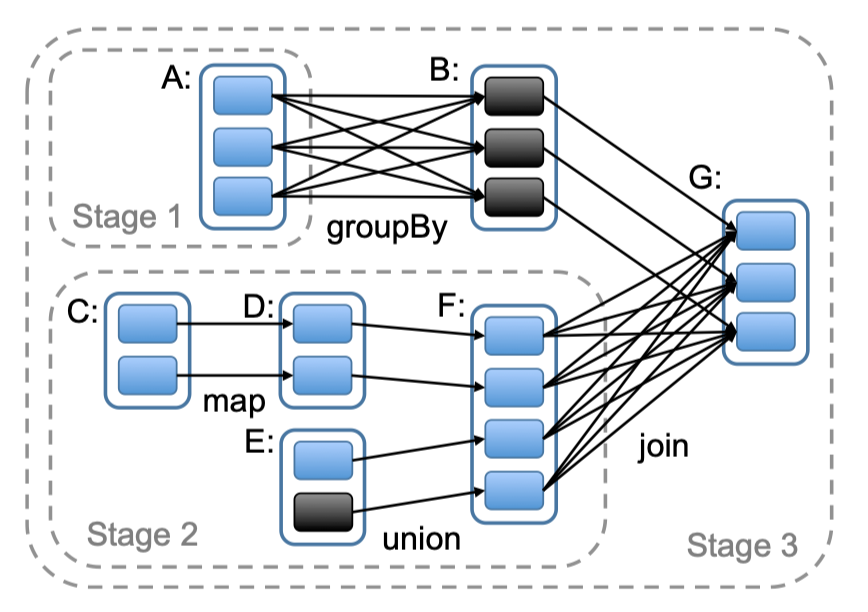
\includegraphics[width=0.55\textwidth]{shuffle-phase-in-spark}
    \caption{Example of how Spark computes job stages. To run an action on RDD
      G, we build build stages at wide dependencies and pipeline narrow
      transformations inside each stage.$^{\text{[Zaharia2012]}}$}
    \label{fig:shuffle-phase-in-spark}
  \end{figure}
\end{frame}

% \begin{frame}
%   \frametitle{Shuffle Phase is Time-consuming}
%   \begin{itemize}
%   \item Shuffle data across the stage in a cluster is time-consuming
%     \begin{itemize}
%     \item The entire working set, which is usually a large fraction of the input
%       data, must be transferred across the network.
%     \item It requires many remote files and network I/Os.$^{\text{[Davidson2013]}}$
%     \end{itemize}
%   \end{itemize}
%   \begin{figure}[!b]
%     \centering
%     \includegraphics[width=0.45\textwidth]{shuffling.png}
%     \caption{Shuffle Phase}
%     \label{fig:shuffling}
%   \end{figure}
% \end{frame}

\begin{frame}
  \frametitle{Netty Involves Many Data Copies}
  \begin{itemize}
  \item The latest Apache Spark takes Netty to perform data shuffle.
    \begin{itemize}
    \item Netty is written with Java Sockets.
    \item It needs multiple data copies and CPU involvement.
    \item It could not fully take advantage of the performance benefits provided
      by high-speed interconnects.
    \end{itemize}
  \end{itemize}
\end{frame}

\begin{frame}
  \frametitle{What is RDMA?}
  \begin{itemize}
  \item RDMA --- \textbf{R}emote \textbf{D}irect \textbf{M}emory \textbf{A}ccess
  \item ``RDMA'' --- networking technologies that have a software interface with
    three features:
    \begin{enumerate}
    \item Remote DMA
    \item Asynchronous work queues
    \item Kernel bypass
    \end{enumerate}
  \item InfiniBand / RoCE(RDMA over Converged Ethernet) / iWARP, etc.
  \item RDMA is increasing its presence in datacenters as the hardware becomes
    cheaper.$^{\text{[Mitchell2013]}}$
  \end{itemize}
\end{frame}

\section{RDMA-based Shuffle Design}

\subsection{Architecture Overview}

\begin{frame}
  \frametitle{Challenges}
  \begin{itemize}
  \item how to keep the existing Spark interface intact?
    \begin{itemize}
    \item adapt the plugin based approach
    \end{itemize}
  \item how to reduce the overhead of RDMA memory registration?
    \begin{itemize}
    \item use tiering memory pool
    \end{itemize}
  \end{itemize}
\end{frame}

\begin{frame}
  \frametitle{Architecture Overview}
  \begin{itemize}
  \item Choosing the plugin based approach to extend current shuffle framework
    in Spark:
    \begin{itemize}
    \item Accelerate Spark workloads using RDMA technology
    \item Keep the existing Spark architecture and interface intact
    \item Can benefit existing Spark applications transparently
    \end{itemize}
  \end{itemize}
\end{frame}

\begin{frame}
  \frametitle{Architecture Overview}
  \begin{itemize}
  \item Redesign the communication layer of Spark shuffle with RDMA
  \item A hybrid approach:
    \begin{itemize}
    \item [1.] using RDMA for data shuffle via Java Native Interface (JNI)
    \item [2.] all other Spark operations go through the Netty module
    \end{itemize}
  \end{itemize}
  \begin{figure}[!b]
    \centering
    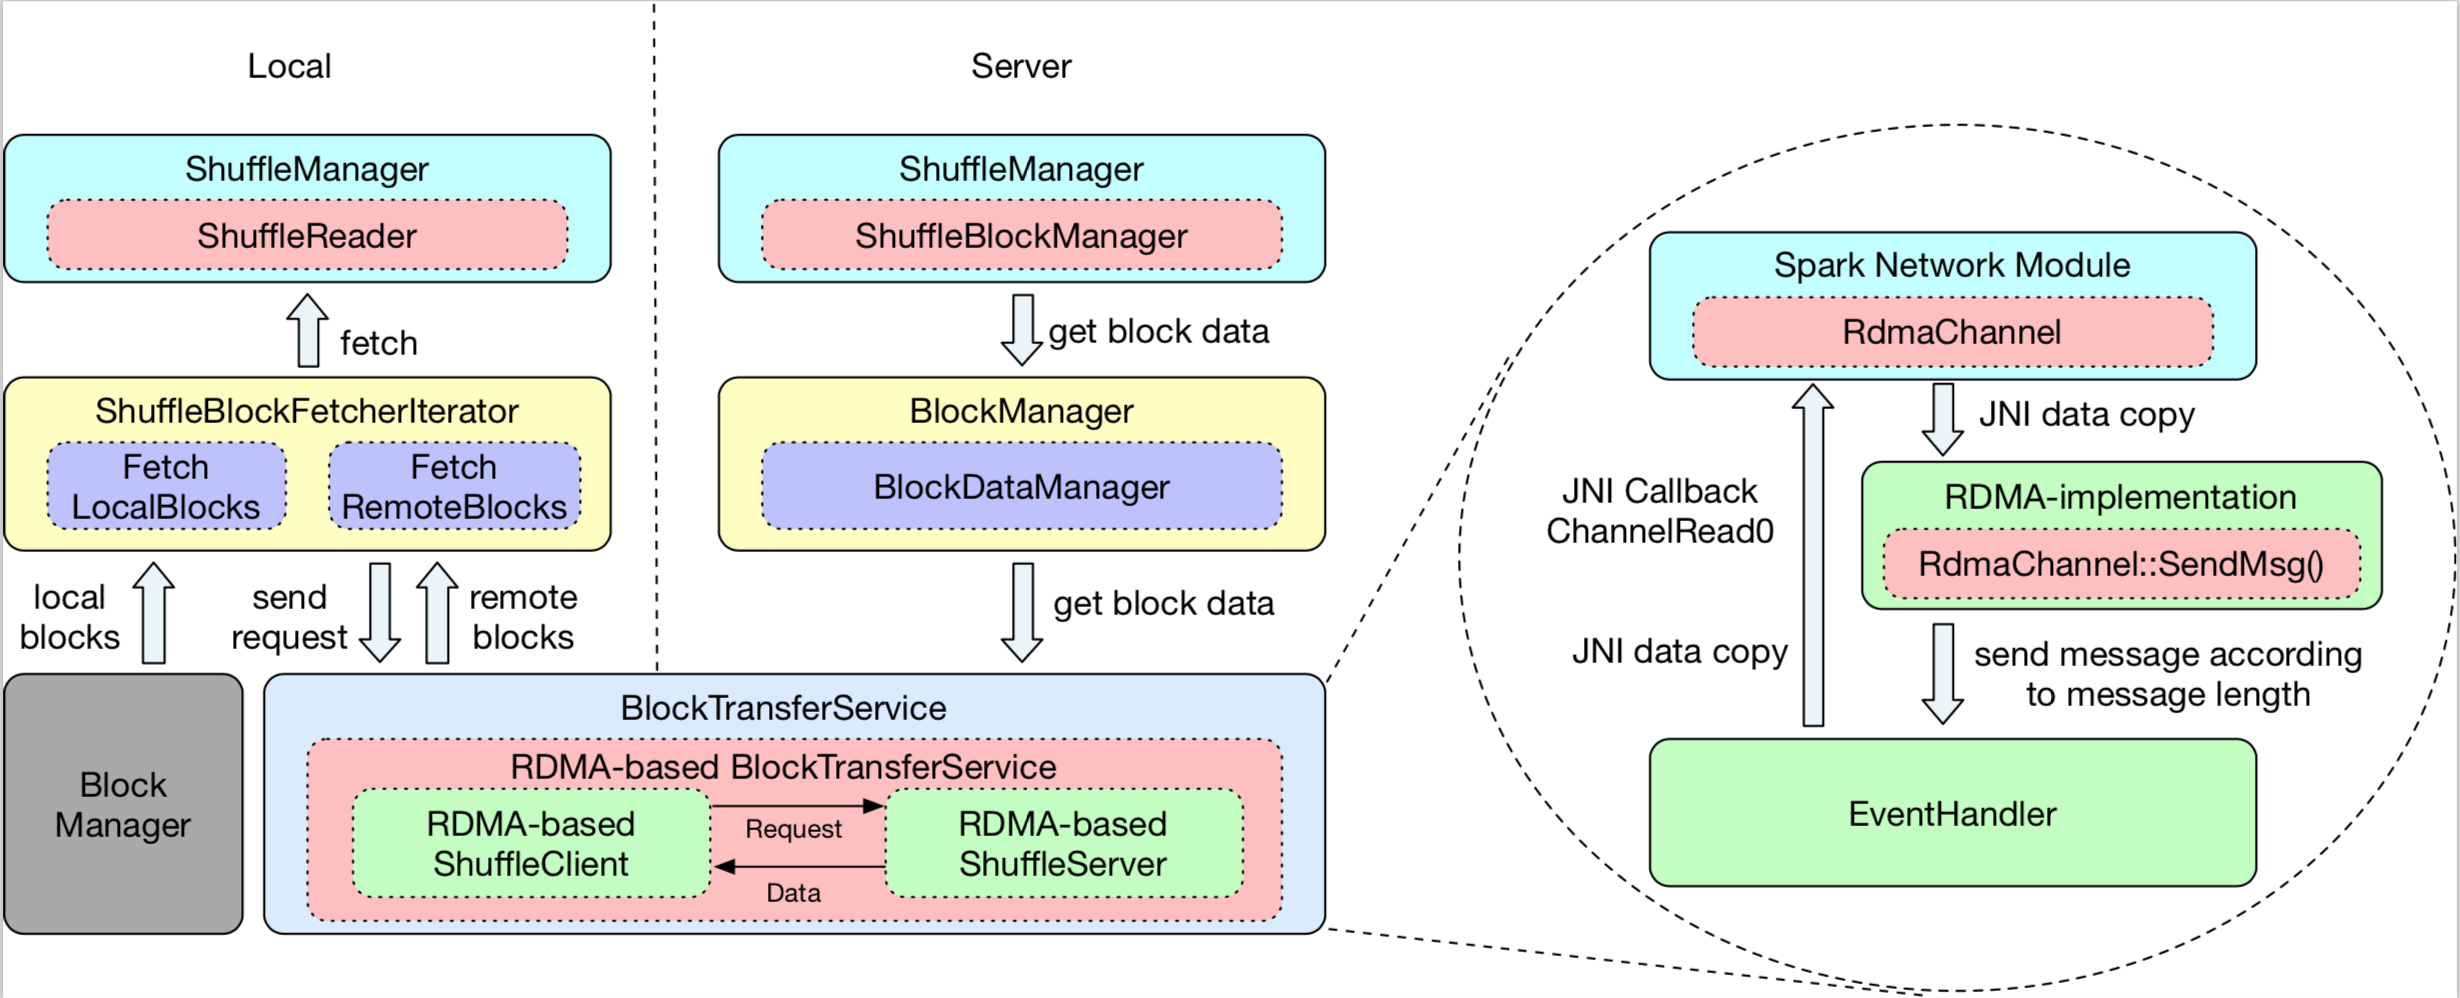
\includegraphics[width=0.85\textwidth]{shuffle-data-flow.png}
    \caption{Flow of RDMA-based data shuffle in Spark.}
    \label{fig:shuffle-data-flow}
  \end{figure}
\end{frame}

\subsection{Design of RDMA-based Data Shuffle}

\begin{frame}
  \frametitle{Major features of our RDMA-based design}
  \begin{enumerate}
  \item RDMA Connection Established
  \item Tiering Memory Pool: avoid frequent memory allocation
  \item Out-of-order Data Transmission: transfer messages of different size
    using different mechanisms
  \end{enumerate}
\end{frame}

\begin{frame}
  \frametitle{Tiering Memory Pool}
  \begin{itemize}
  \item using RDMA for data transmission requires registering memory to RNIC
  \item and the operation of registering and deregistering memory includes a
    significant overhead$^{\text{[Frey2009]}}$
  \item We use \textit{boost.pool} to implement a tiering memory pool.
  \end{itemize}
\end{frame}

\begin{frame}
  \frametitle{Tiering Memory Pool}
  \begin{itemize}
  \item registering a large piece of memory in advance, with the chunk\rq{s}
    size ranging from 32B, 1KB, 32KB, 1MB and 32MB
  \item implement our own allocator, including \textit{malloc} and \textit{free}
    \begin{itemize}
    \item \textit{malloc} --- allocate memory and register memory
    \item \textit{free} --- only called when application finished
    \end{itemize} 
  \end{itemize}
  \begin{figure}[!b]
    \centering
    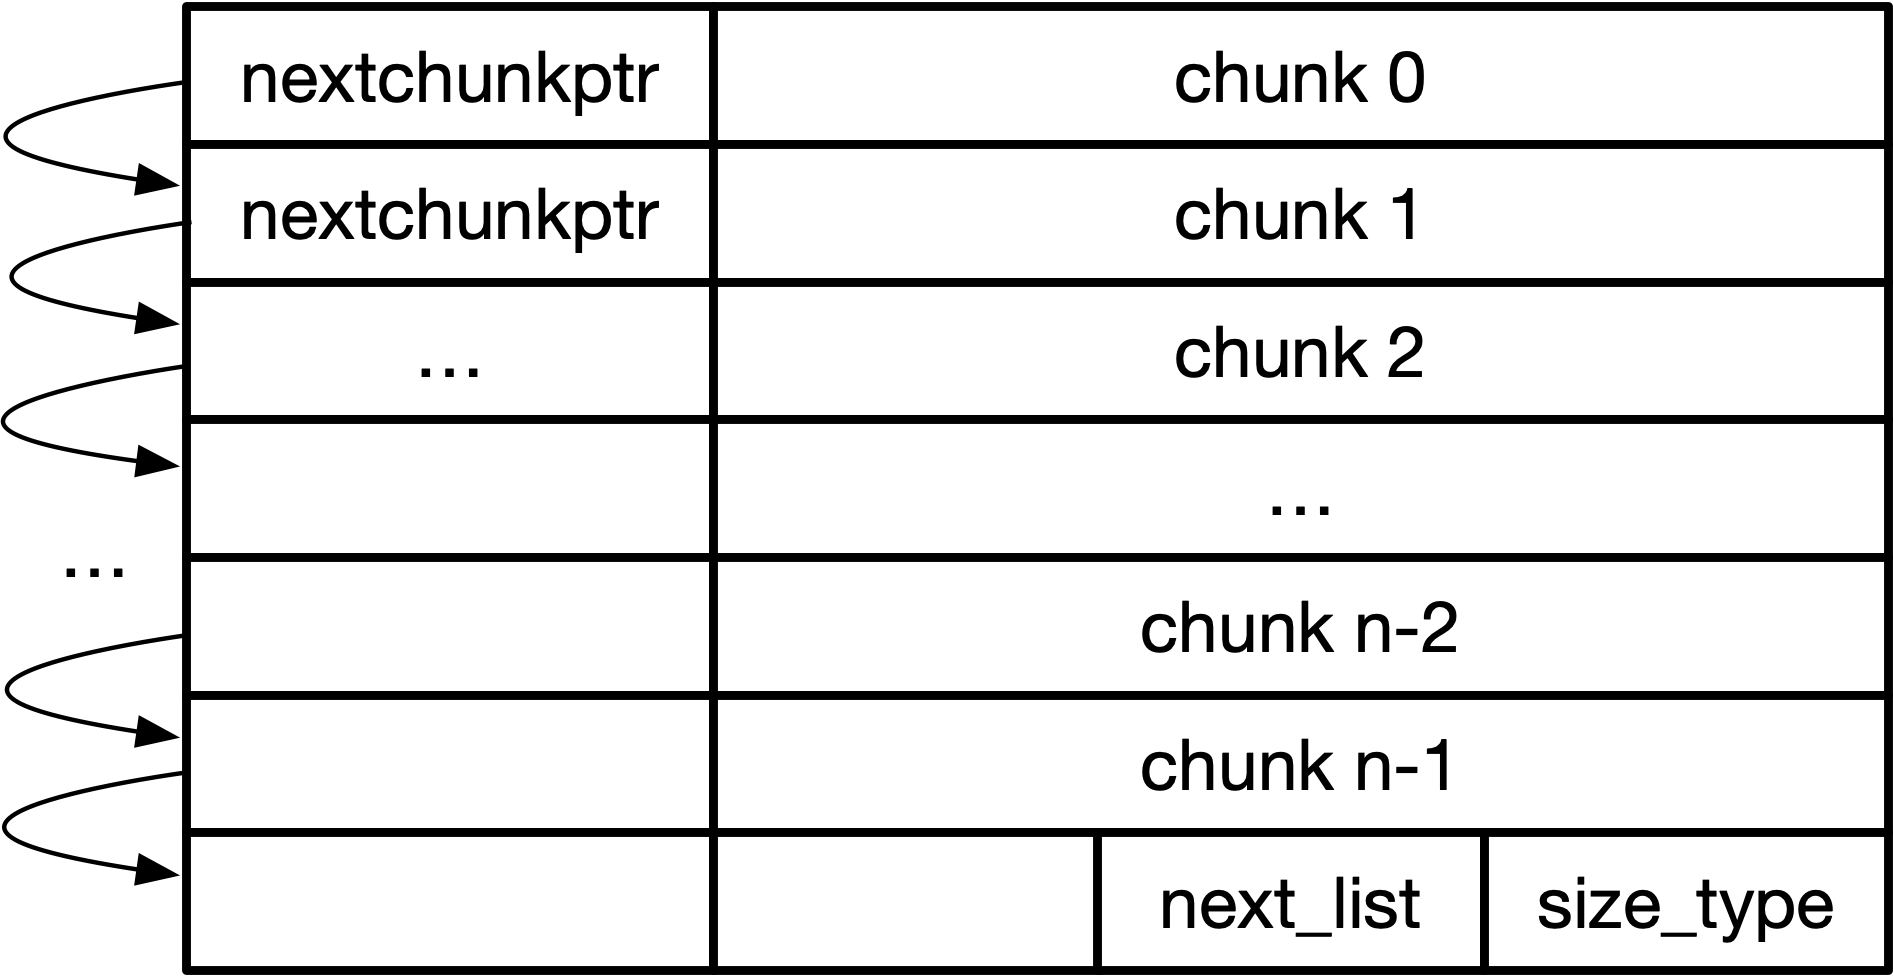
\includegraphics[width=0.6\textwidth]{boost-pool.png}
    \caption{Block and chunks in boost.pool.}
    \label{fig:boost-pool}
  \end{figure}
\end{frame}

\begin{frame}
  \frametitle{Out-of-order Data Transmission}
  \begin{itemize}
  \item use the unique id to ensure data processing correctly
  \item choose a threshold value to divide messages into small and large
    \begin{itemize}
    \item in the experiment section, we hard-code 1KB
    \end{itemize}
  \item for small messages, we just use two-side SEND/RECV
  \item for large messages, we use one-side READ
  \item NOW, we are working with WRITE and WRITE\_WITH\_IMM.
  \end{itemize}
\end{frame}

\begin{frame}
  \frametitle{Data Transfer procedure}
  \begin{figure}[!b]
    \centering
    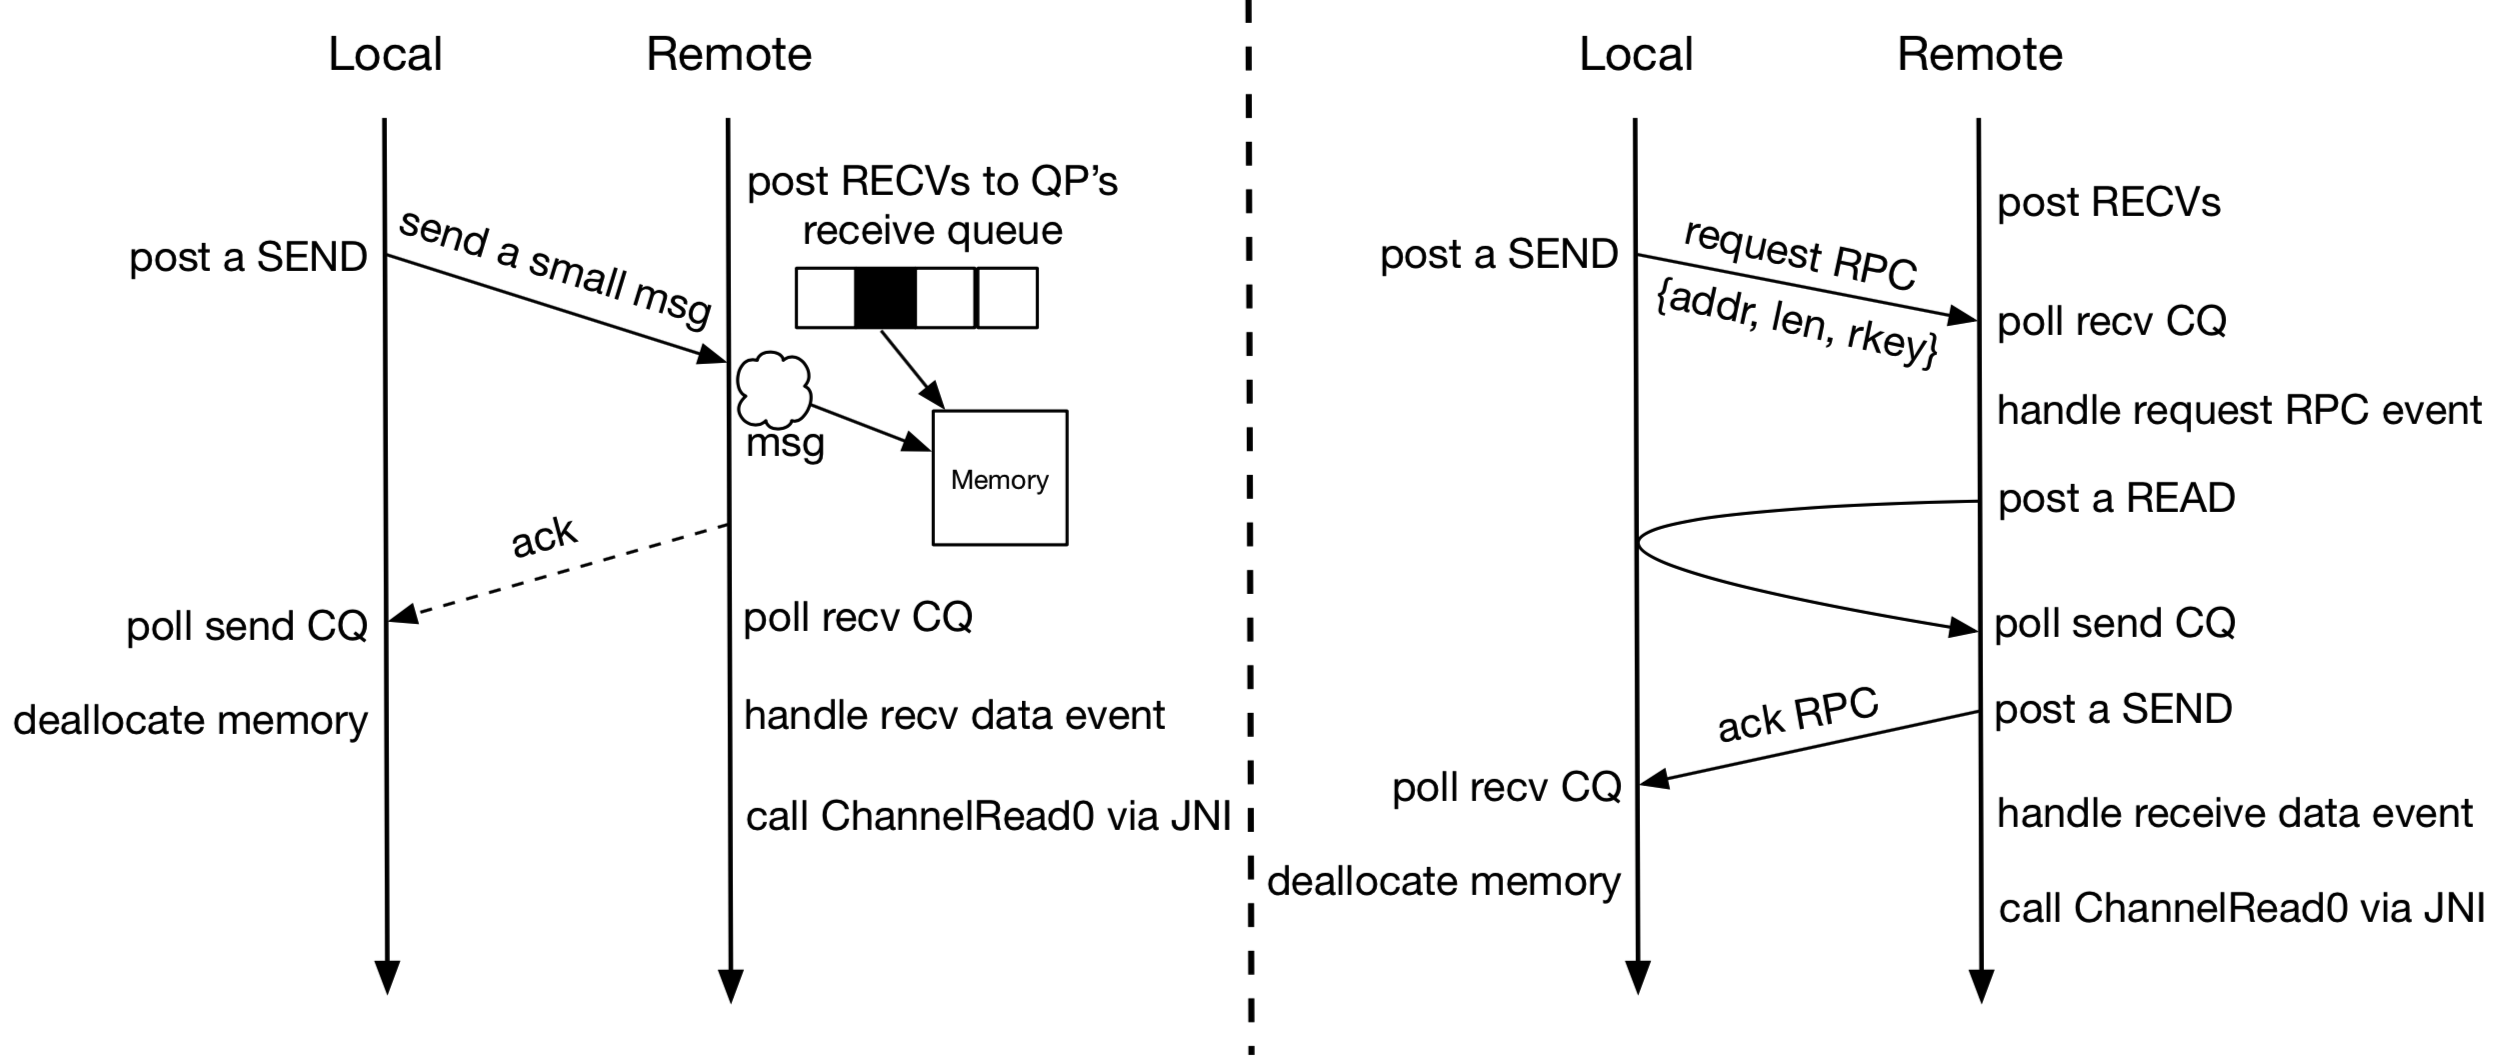
\includegraphics[width=0.9\textwidth]{data-procedure.png}
    \caption{The data transfer procedure.}
    \label{fig:data-procedure}
  \end{figure}
\end{frame}


\section{Evaluation}

\begin{frame}
  \frametitle{Setup}
  \begin{itemize}
  \item All of our experiments are conducted on a small cluster of 5 machines.
    One is master and the other is worker.
  \end{itemize}
  \begin{table}[!b]
    \centering
    \begin{tabular}{l|l}
    \hline
    CPU & 2.10~GHz Intel Xeon E5-2620L 6-core processors \\
    OS & Red Hat Enterprise Linux Server 6 with kernel 2.6.32 \\
    Connections & InfiniBand FDR using Mellanox MT27500\\
                & ConnectX-3 HCA (40Gb/s) and 1Gb/s Ethernet \\
    Memory & 128~GB \\
    Hard Disk & 2~TB \\
    Spark Version & 1.6.0 \\
    Hadoop Version & 2.7.3 \\
    \hline
    \end{tabular}
    \caption{Environment setup.}
    \label{tab:setup-environment}
  \end{table}
\end{frame}

\begin{frame}
  \frametitle{Comparison with}
  \begin{enumerate}
  \item our RDMA-based Shffule design
  \item the default Spark based on Netty over IPoIB
  \item Crail-Spark-IO --- a recent open-source Spark shuffle plugin from IBM
    \begin{itemize}
    \item based on DaRPC$^{\text{[stuedi2014]}}$
    \item using Spark 2.0.0 to meet its building requirements
    \end{itemize}
  \end{enumerate}
\end{frame}

\begin{frame}
  \frametitle{Crail-Spark-IO}
  \begin{itemize}
  \item shuffle operation becomes as simple as writing and reading files
  \end{itemize}
  \begin{figure}[!b]
    \centering 
    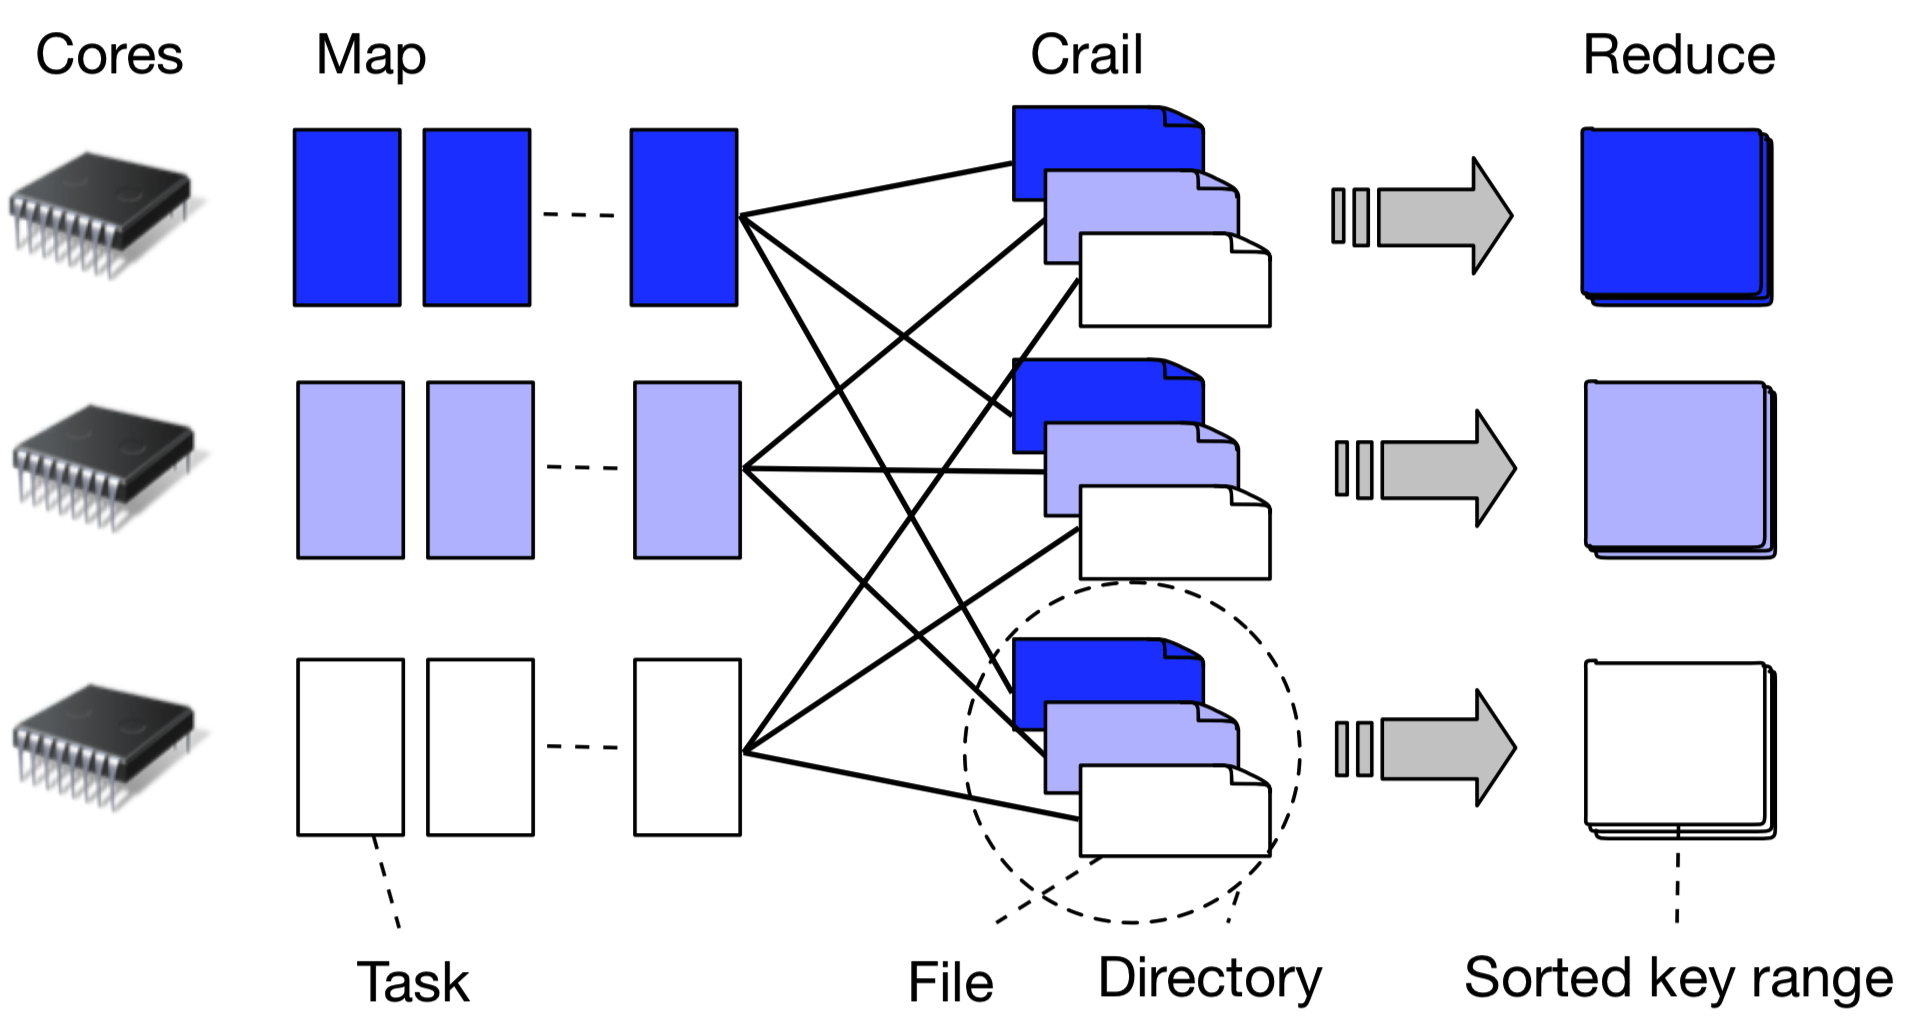
\includegraphics[width=0.75\textwidth]{crail-shuffle-module.png}
    \caption{The Crail shuffle module.$^{\text{[Stuedi2017]}}$}
    \label{fig:crail-shuffle-module}
  \end{figure}
\end{frame}

\begin{frame}
  \frametitle{Workloads}
  \begin{itemize}
  \item We have chosen four workloads in two categories:
    \begin{enumerate}
    \item RDD benchmarks (GroupBy and SortBy)
    \item Iterative algorithms (TriangleCount and SVM in
      SparkBench$^{\text{[Li2015]}}$)
    \end{enumerate}
  \end{itemize}
\end{frame}

\begin{frame}
  \frametitle{Evaluation of Shuffle Read Block Time}
  \begin{itemize}
  \item Shuffle Read Block Time --- the time that tasks spent blocked waiting
    for shuffle data to be read from remote machines
    \item In general, compared with the Netty-based shuffle design, the
      RDMA-based shuffle design performs better.
  \end{itemize}
  \begin{figure}[!b]
    \centering 
    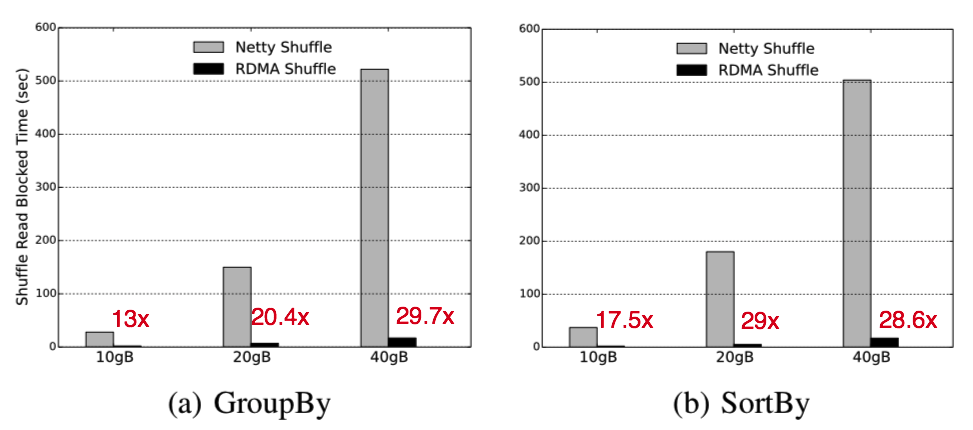
\includegraphics[width=0.65\textwidth]{shuffle-read-block-time.png}
    \caption{Shuffle read blocked time evaluation for GroupBy and SortBy.}
    \label{fig:shuffle-read-block-time}
  \end{figure}
\end{frame}

\begin{frame}
  \frametitle{Performance Evaluation of RDD Benchmarks}
  \begin{itemize}
  \item RDMA-based design performs better than the default design
  \item Compared with Crail-Spark-IO, our implementation can get 25\% and 9\%
    improvement for GroupBy and SortBy, respectively.
  \end{itemize}
  \begin{figure}[!b]
    \centering 
    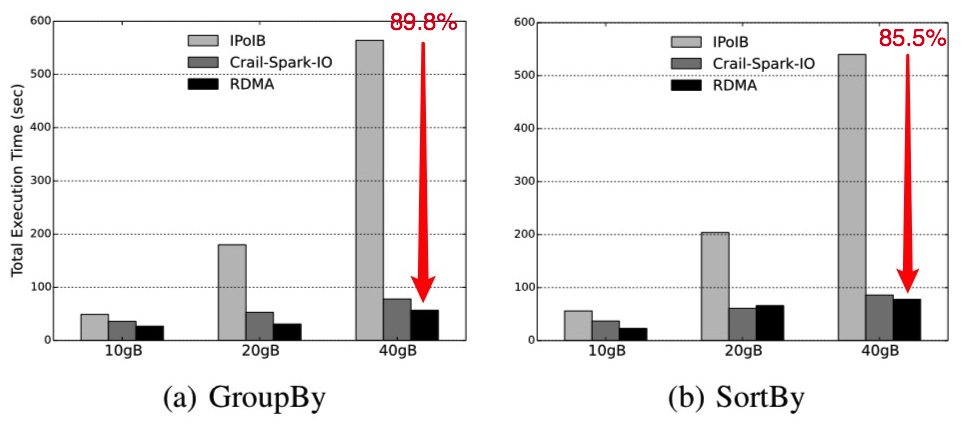
\includegraphics[width=0.65\textwidth]{rdd-benchmarks.png}
    \caption{Performance evaluation for RDD benchmarks.}
    \label{fig:rdd-benchmarks}
  \end{figure}
\end{frame}

\begin{frame}
  \frametitle{Performance Evaluation with Iterative Algorithms}
  \begin{itemize}
  \item RDMA-based design performs better than the default design.
  \item Compared with Crail-Spark-IO, when the data size is small, we can get about 41\% and 44\% improvement for 1gB and 2gB.
  \item In SVM, when data size is 10gB, the shuffle data is small.
  \end{itemize}
  \begin{figure}[!b]
    \centering 
    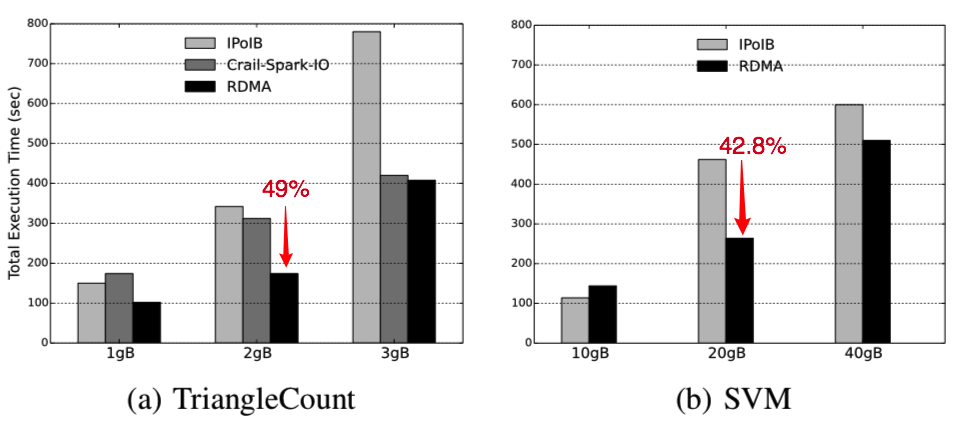
\includegraphics[width=0.65\textwidth]{iterative-algorithms.png}
    \caption{Performance evaluation for iterative algorithms.}
    \label{fig:iterative-algorithms}
  \end{figure}
\end{frame}

\section{Summary}

\begin{frame}
  \frametitle{Summary}
  \begin{itemize}
  \item Shuffling phase is time-consuming because it requires many remote files
    and network I/Os.
  \item RDMA enables zero-copy transfers, reducing latency and CPU overhead.
  \item A hybrid approach that incorporates communication over conventional
    sockets as well as RDMA over InfiniBand:
    \begin{enumerate}
    \item tiering memory pool --- avoid frequent memory allocation
    \item SEND/RECV and READ --- transfer small and large messages
    \end{enumerate}
  \item Our accelerations to the data transfer layer through this
    RDMA-based shuffle can benefit Spark workloads transparently.
  \end{itemize}
\end{frame}

\begin{frame}[plain]
  \frametitle{}
  {
    \LARGE{
      \bfseries
      \begin{center}
        Thank you!
      \end{center}
    }
  }
\end{frame}

\end{document}